\section{Modelos Treinados} \label{modelos_treinados}
Nesta secção vai-se falar de todos os modelos treinados, das motivações para o treinamento dos mesmos, e o que o grupo achou dos resultados que o mesmo ofereceu de um ponto de vista prático, sendo realizada na secção \ref{avaliacoes_dos_modelos} uma análise mais analítica sobre os mesmos.

\subsection{Modelos para o PokeMMO}
\subsubsection{Primeiro Modelo}
Como foi descrito na secção \ref{tarefas_a_automatizar}, os modelos foram treinados com base no modelo de deteção de objetos YOLO, sendo utilizada a versão 8 neste projeto, que é a versão mais recente, não experimental, disponibilizada pelo \textit{ultralytics}, no entanto, o mesmo tem diferentes versões menos capacitadas dentro de uma mesma versão, para poder adequar-se a hardwares mais limitados. Antes da realização do trabalho, já se tinha treinado um modelo com o YOLOv8n, a versão mais limitada, para o jogo \textit{Forge of Empires}, mas a mesma mostrou-se bastante ineficiente, para além de mostrar que o grupo tinha poder computacional para suportar modelos mais pesados.

Para este primeiro modelo, para o PokeMMO, decidiu-se treinar o modelo com o \textit{YOLOv8m}, que é uma versão muito mais competente comparativamente ao \textit{YOLOv8n}, mas estando muito longe de ser a melhor o melhor modelo que a versão 8 oferece. Após realizar o treino, que provou estar no limite das capacidades computacionais do grupo, o grupo ficou muito satisfeito com os resultados obtidos, as imagens passadas para o modelo conseguiam detetar quase sempre as informações pretendidas.

\begin{figure}[h]
    \centering
    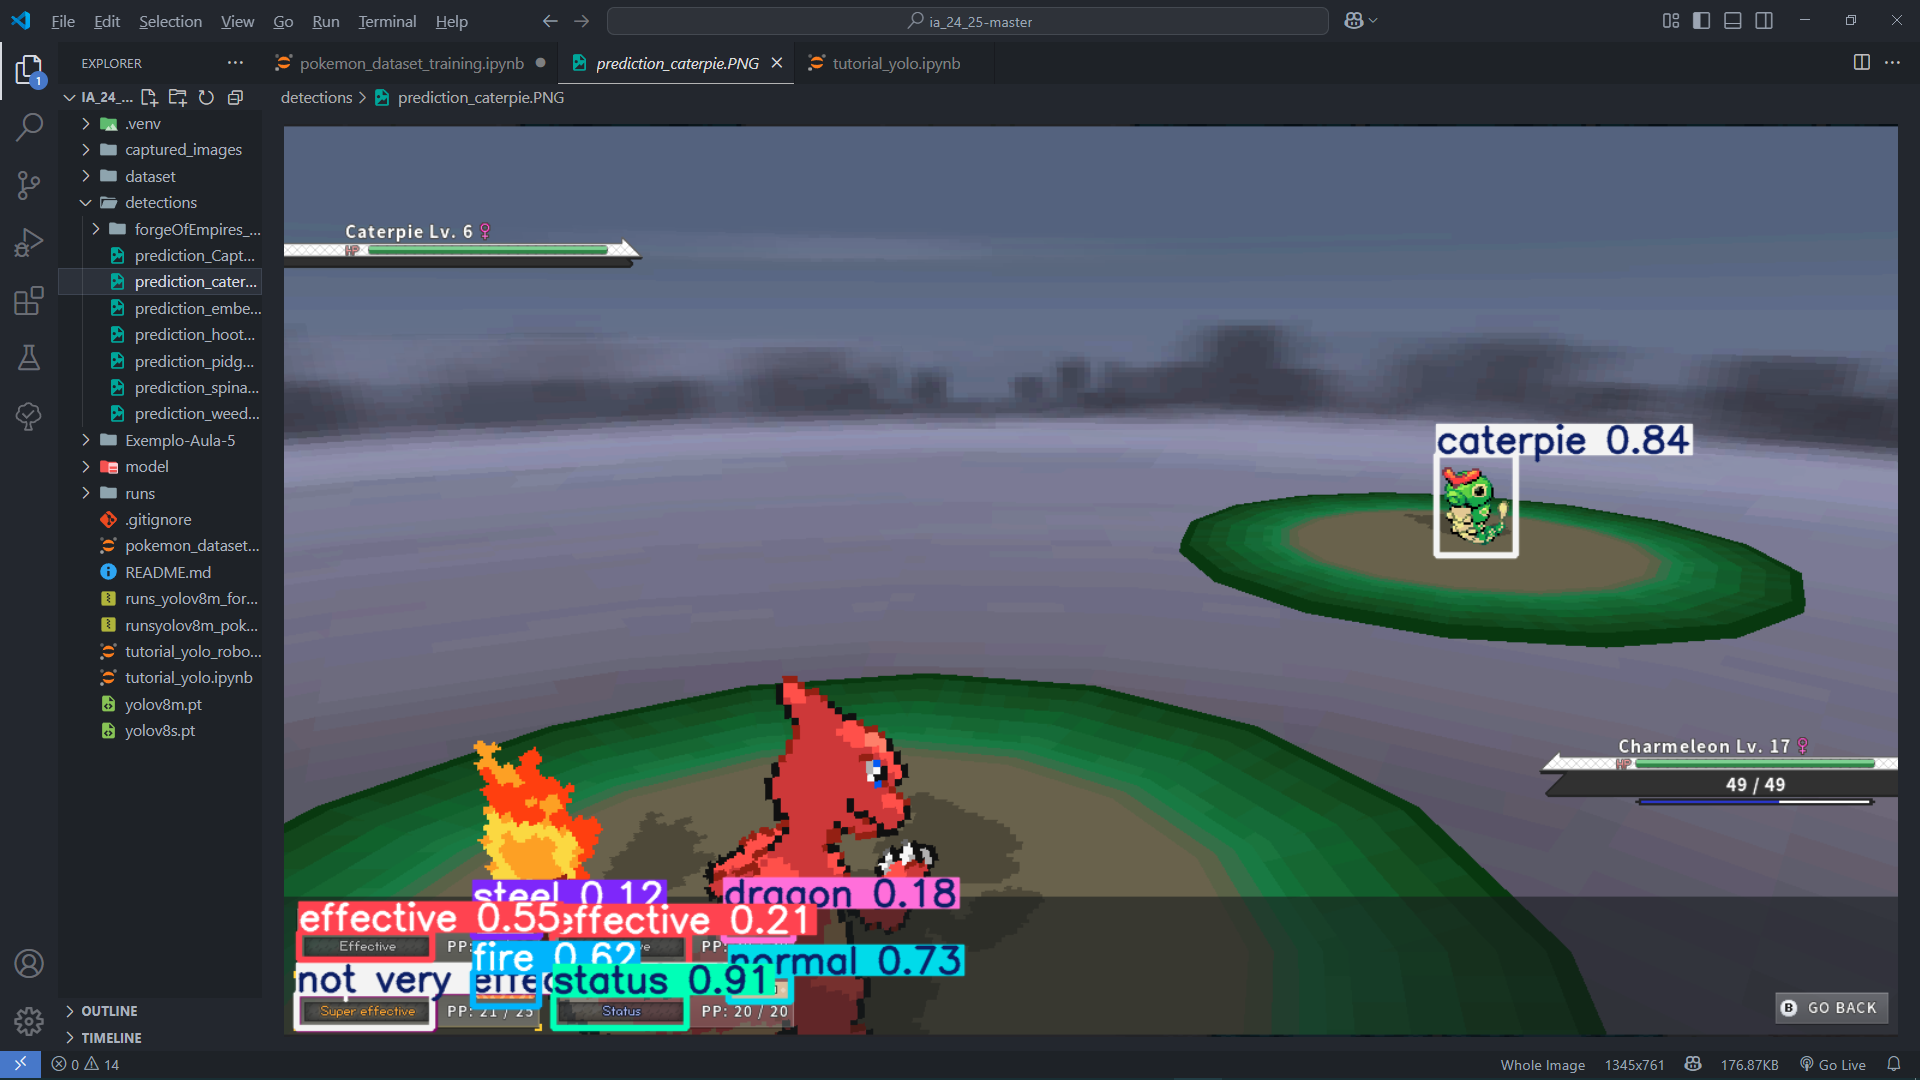
\includegraphics[width=0.7\linewidth]{imagens/primeiro_modelo_exemplo.png}
    \caption{Imagem resultante do primeiro modelo para o PokeMMO}
    \label{fig:primeiro_modelo_exemplo}
\end{figure}

\subsubsection{Segundo Modelo}
Mesmo com os resultados satisfatórios do primeiro modelo treinado, decidiu-se treinar uma nova versão do modelo, mas desta vez com o \textit{YOLOv8x}, que é a melhor versão oferecida pelo \textit{YOLOv8}, no entanto, como o grupo não tinha a capacidade de realizar um treino com esta versão, então recorreu-se à plataforma Kaggle, que permite a execução de notebooks online, possibilitando assim o treinamento de modelos mais pesados.

Num ponto de vista prático, não se conseguiu ver muitas diferenças entre a versão $m$ e a versão $x$ do \textit{YOLOv8}, as imagens devolvidas pelo modelo continuavam a ter um resultado bastante satisfatório, mas não ausente de falsos positivos nem falsos negativos, e também não pareceu haver uma diminuição da ocorrência dos mesmos. No entanto, após tentar levar este modelo para um ambiente de produção, o modelo quase não funcionava, como foram treinadas imagens só com o ecrã de combate, ignorando o resto da interface, o modelo pouco conseguia prever, as informações estavam bastante pequenas para o modelo conseguir detetar, para além de haver muita movimentação tanto da câmara do jogo, como do sprite do Pokémon adversário, dificultando ainda mais a previsão.

Infelizmente não existe forma de aumentar o tamanho do ecrã de batalha nas definições do jogo, e muito provavelmente o problema iria continuar a ocorrer mesmo que se treina-se um novo modelo mas desta vez com imagens do ecrã todo, pois  muitas das informações a recolher já eram pequenas no dataset original, sendo a principal fonte de falsos negativos, logo ao treinar um novo dataset com a totalidade do ecrã pouco iria resolver, portanto decidiu-se trocar de jogo.

\subsection{Modelos para o Pokémon HeartGold}
\subsubsection{Primeiro Modelo}
Após analisar os problemas dos modelos anteriores, chegou-se à conclusão que a série de jogos Pokémon continuava a ser uma boa escolha para o trabalho a desenvolver, o grupo precisava apenas escolher um jogo que se iria adaptar melhor às limitações dos modelos de imagens, então decidiu-se criar um novo dataset mas desta vez para o jogo Pokémon HeartGold, pois como este é um jogo de Nintendo DS, o grupo vai estar sempre limitado à resolução nativa do ecrã do Nintendo DS, e como esta consola tinha um ecrã sensível ao toque, permitia uma fácil execução num ambiente de produção.

Após realizar a recolha, etiquetagem e o treino com o modelo \textit{YOLOv8x}, os resultados obtidos foram bastante satisfatórios. O modelo demonstrou um desempenho muito consistente, com uma taxa reduzida de erros. No entanto, identificou-se um problema recorrente na deteção do botão de "luta". Sempre que o fundo da imagem era predominantemente preto, o modelo tendia a reconhecer essas áreas como sendo o botão de "luta", mesmo quando este não estava presente. Apesar dessas deteções apresentarem geralmente um nível de confiança baixo, e por isso terem impacto reduzido num ambiente de produção, o grupo considerou importante perceber a origem do erro.

Após discutir com o professor da unidade curricular, concluiu-se que o modelo não estava a aprender a identificar o botão com base na cor, mas sim na sua forma retangular. Assim, qualquer área escura com formas semelhantes acabava por ser identificada erroneamente. Para mitigar este tipo de erro, optou-se por aplicar técnicas de \textit{data augmentation}, que permitiram aumentar a robustez do modelo e melhorar a sua capacidade de generalização. As técnicas utilizadas estão descritas com mais detalhe na Secção \ref{data_augmentation}

\begin{figure}[h]
    \centering
    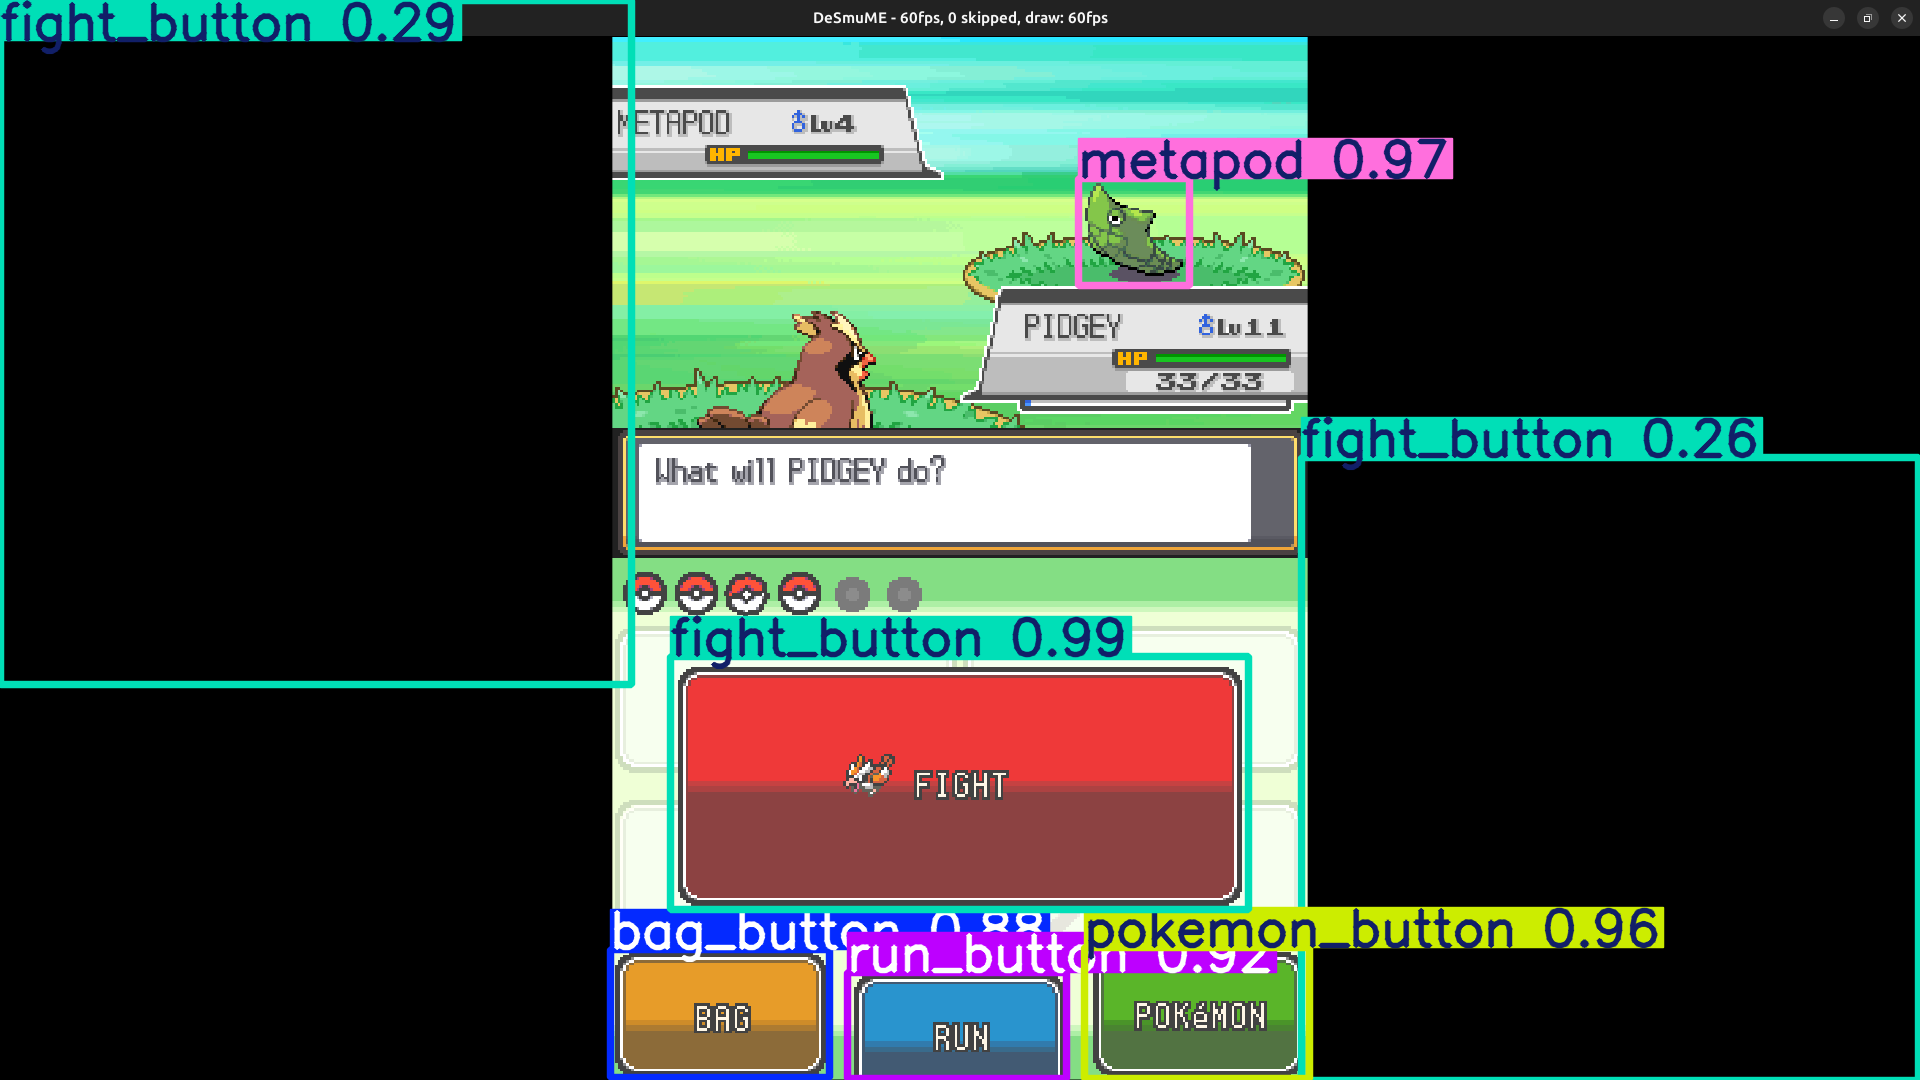
\includegraphics[width=0.8\linewidth]{imagens/phg_fight_button.png}
    \caption{Informações recolhidas do primeiro modelo do Pokémon HeartGold}
    \label{fig:phg_primeiro_modelo}
\end{figure}

Nesta primeira versão do dataset apenas etiquetou-se no roboflow o tipo dos ataques, e não o ataque como um todo, logo o modelo não sabe que ataque está a usar, então para implementar esta primeira versão do modelo, que até então era para ser a definitiva, num ambiente de produção, fez-se um dataset em formato \textit{csv} com a efetividade dos determinados tipos de ataques contra alguns Pokémons presentes no dataset, e treinou-se uma árvore de decisão que iria escolher o ataque que o Pokémon iria usar contra o adversário consoante o tipo do ataque. Como não se sabe o que o ataque faz, esta abordagem acaba por ter vários problemas no combate, porque muitas vezes o modelo previa um determinado ataque como o melhor contra o Pokémon adversário, no entanto, como apenas levou o tipo do ataque em consideração, estava apenas a aplicar buffs (Bónus) a si mesmo ou debuffs (penalizações) ao inimigo, não infringindo dano.

\begin{figure}[h]
    \centering
    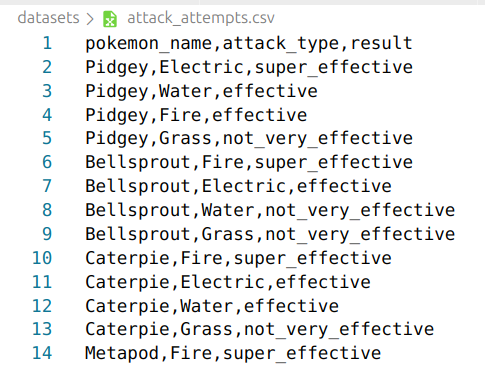
\includegraphics[width=0.5\linewidth]{imagens/dataset_ataques.png}
    \caption{Dataset de efetividade de tipos}
    \label{fig:phg_segundo_modelo}
\end{figure}

\subsubsection{Modelo Final}
Nesta versão do modelo, para além da aplicação de técnicas de \textit{data augmentation}, decidiu-se também recolher mais informações das lutas. Para isso, procedeu-se à identificação dos níveis dos Pokémons em batalha, bem como os nomes dos ataques, com o objetivo de localizar as áreas onde esses elementos estavam presentes. Posteriormente, recorreu-se a uma ferramenta de reconhecimento ótico de caracteres (OCR) para ler essas áreas e, assim, permitir ao bot tomar a melhor decisão com base na informação extraída.

Inicialmente, foi testado o \textbf{Tesseract}, um motor de OCR de código aberto. No entanto, este mostrou-se ineficaz na leitura de texto pixelizado, apresentando resultados fracos na identificação do conteúdo do ecrã.

Seguidamente, utilizou-se o \textbf{EasyOCR}, uma biblioteca de OCR baseada em deep learning, que oferece suporte a múltiplas línguas e é conhecida pela sua simplicidade de utilização. Embora ainda apresentasse alguns erros na leitura dos nomes dos Pokémon e dos ataques, e não conseguisse identificar corretamente os níveis dos Pokémons, representou uma melhoria significativa em relação ao \textit{Tesseract}.

Por fim, foi experimentado o \textbf{Granite}, uma solução mais avançada de OCR baseada em modelos modernos de visão por computador. Contudo, os resultados obtidos não trouxeram melhorias relevantes face ao \textit{EasyOCR} e o tempo de execução era significativamente superior. Dado esse fator, optou-se por manter o \textit{EasyOCR} como ferramenta principal para esta tarefa.

Devido à elevada variabilidade e frequência de erros ortográficos nas informações extraídas, considerou-se inviável treinar um modelo tradicional para a tomada de decisões. Assim, optou-se pela utilização de um modelo de linguagem (LLM) local, executado através do \textit{Ollama}, que permite interpretar e decidir com base em texto imperfeito. Inicialmente foi testado o modelo \textbf{TinyLlama}, mas este não seguia de forma fiável as instruções fornecidas. Portanto decidiu-se experimentar os modelos \textbf{Phi2}, \textbf{Phi4}, \textbf{Deepseek-v2}, sendo que, no final, o modelo que melhor se adequou às exigências do projeto, seja ao nível de respostas como ao nível de desempenho, foi o \textbf{Mistral}.

Embora o modelo ainda apresente algumas limitações na interpretação de certas entradas, os resultados obtidos são, de forma geral, bastante satisfatórios. A sua capacidade de lidar com dados ruidosos e tomar decisões coerentes torna-o suficientemente robusto para ser utilizado em ambiente de produção.

\begin{figure}[h]
    \centering
    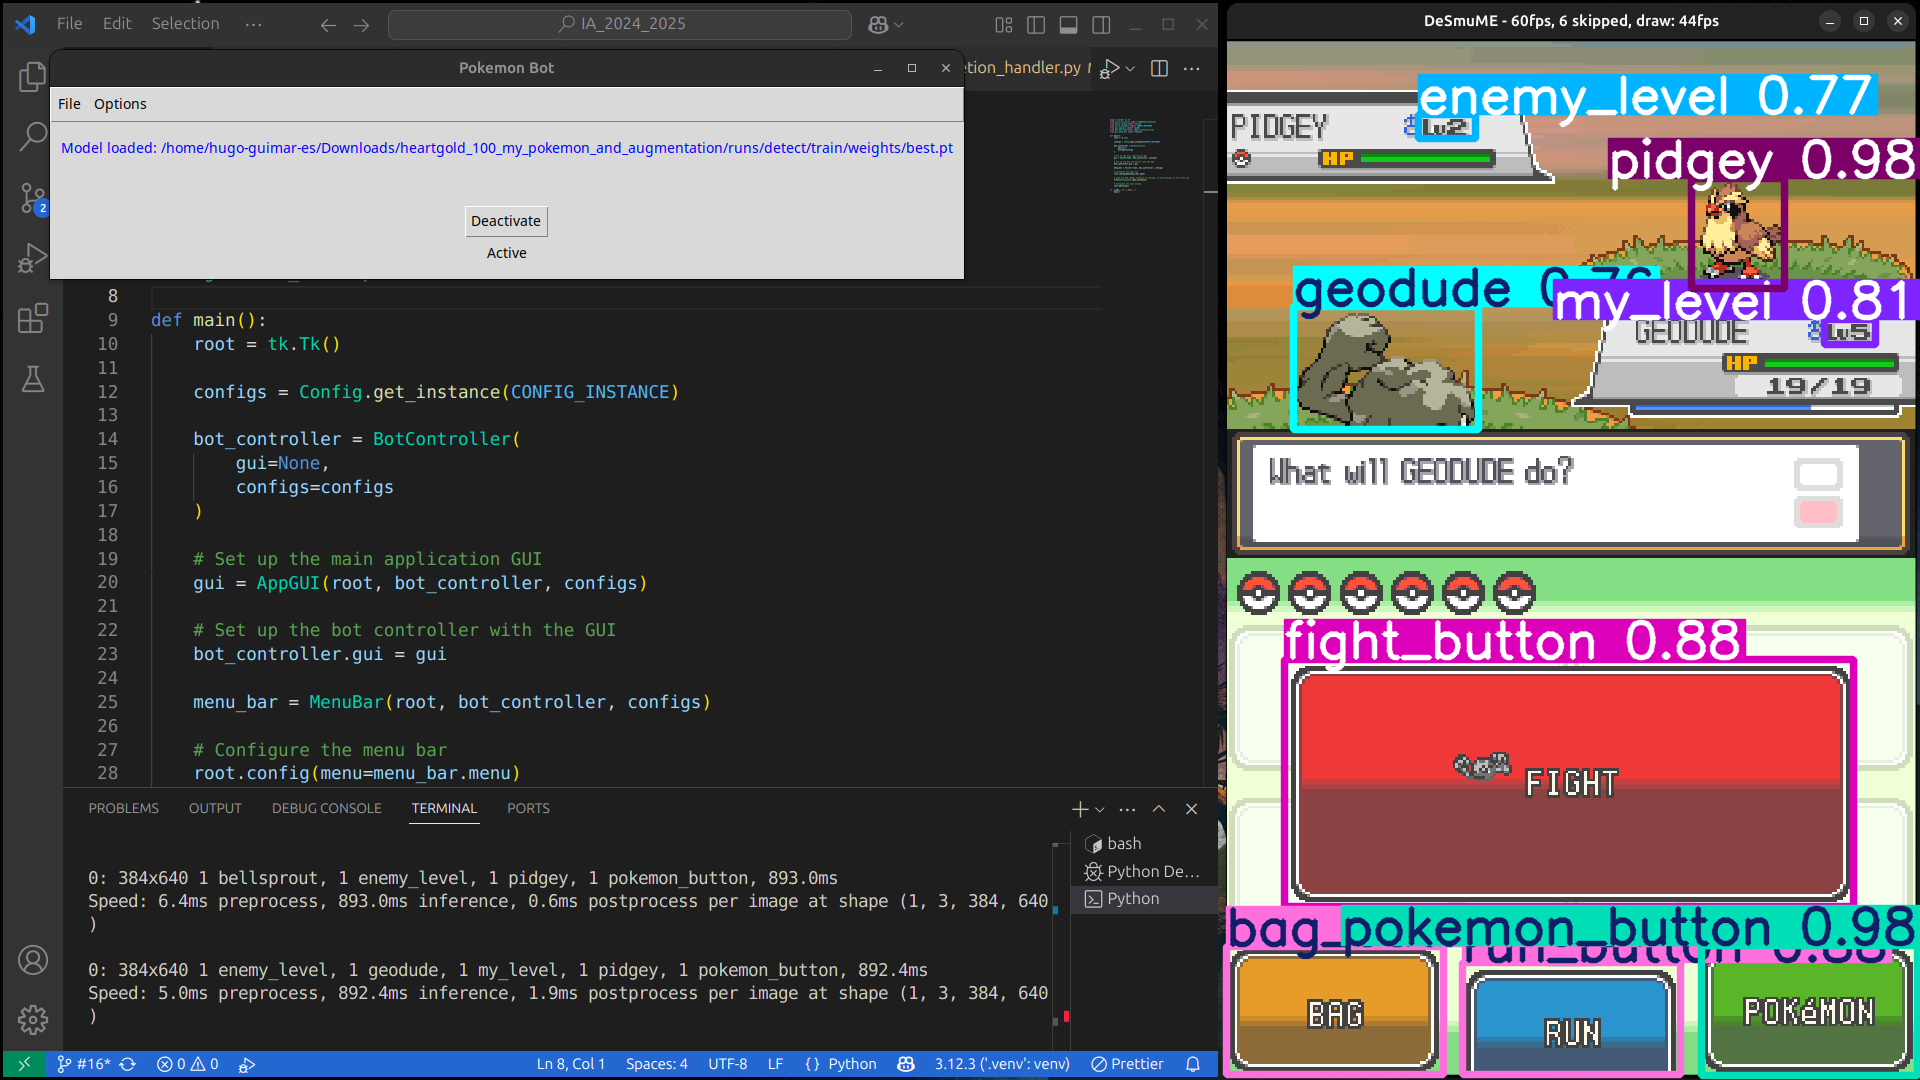
\includegraphics[width=1.0\linewidth]{imagens/informacoes_modelo_final.png}
    \caption{Informações recolhidas pelo modelo final em produção}
    \label{fig:infomacoes_modelo_final}
\end{figure}